\documentclass[../LogosReference.tex]{subfiles}
\begin{document}

% ============================================================================
% Section: Introduction
% ============================================================================

\section{Introduction}\label{sec:introduction}

A semantic frame provides the primitive structures used to interpret a formal language. Extending the expressive power of a language requires strategic extensions to the primitive semantic resources provided by the frame, including precisely the resources needed and nothing more. This ensures that language and frame remain in perfect step with each other.

This reference manual provides the formal specification of the Logos logic system. The semantics proceeds through increasingly expressive extensions, each extending the frame and evaluation mechanisms of the previous.

% ------------------------------------------------------------
% Extension Dependencies
% ------------------------------------------------------------

\subsection{Extension Dependencies}\label{sec:extension-dependencies}

The following diagram shows the dependency structure among extensions:

\begin{center}
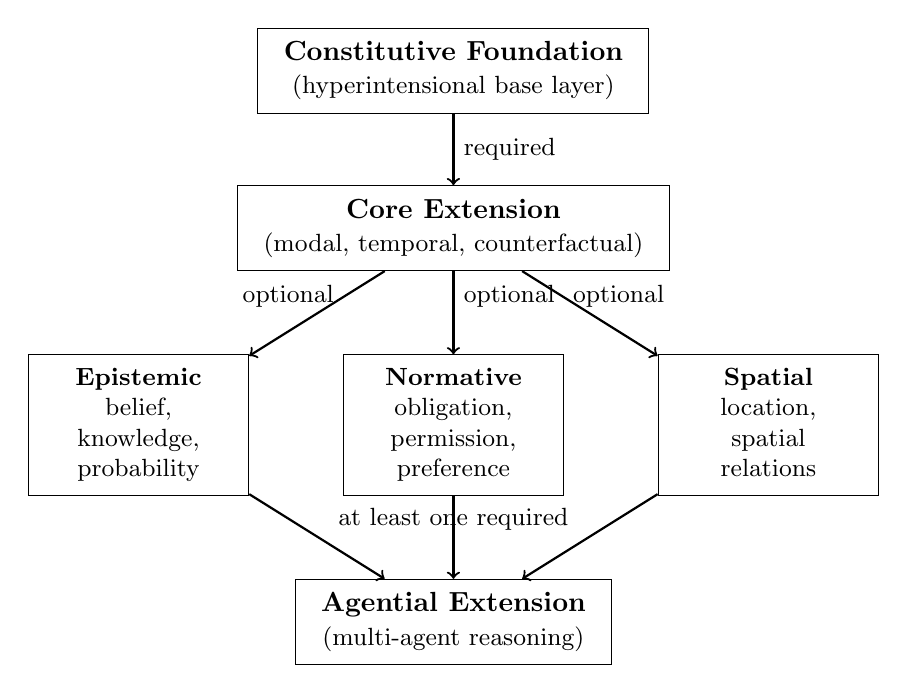
\begin{tikzpicture}[
  box/.style={rectangle, draw, text centered, minimum width=4cm, minimum height=1cm},
  smallbox/.style={rectangle, draw, text centered, minimum width=2.8cm, minimum height=1.5cm, font=\small},
  arrow/.style={->, thick}
]

% Constitutive Foundation
\node[box] (foundation) at (0, 6) {
  \begin{tabular}{c}
    \textbf{Constitutive Foundation} \\
    {\small (hyperintensional base layer)}
  \end{tabular}
};

% Core Extension
\node[box] (core) at (0, 4) {
  \begin{tabular}{c}
    \textbf{Core Extension} \\
    {\small (modal, temporal, counterfactual)}
  \end{tabular}
};

% Middle Extensions
\node[smallbox] (epistemic) at (-4, 1.5) {
  \begin{tabular}{c}
    \textbf{Epistemic} \\
    belief, \\
    knowledge, \\
    probability
  \end{tabular}
};

\node[smallbox] (normative) at (0, 1.5) {
  \begin{tabular}{c}
    \textbf{Normative} \\
    obligation, \\
    permission, \\
    preference
  \end{tabular}
};

\node[smallbox] (spatial) at (4, 1.5) {
  \begin{tabular}{c}
    \textbf{Spatial} \\
    location, \\
    spatial \\
    relations
  \end{tabular}
};

% Agential Extension
\node[box] (agential) at (0, -1) {
  \begin{tabular}{c}
    \textbf{Agential Extension} \\
    {\small (multi-agent reasoning)}
  \end{tabular}
};

% Arrows
\draw[arrow] (foundation) -- node[right] {\small required} (core);
\draw[arrow] (core) -- node[left, pos=0.3] {\small optional} (epistemic);
\draw[arrow] (core) -- node[right, pos=0.3] {\small optional} (normative);
\draw[arrow] (core) -- node[right, pos=0.3] {\small optional} (spatial);
\draw[arrow] (epistemic) -- (agential);
\draw[arrow] (normative) -- (agential);
\draw[arrow] (spatial) -- (agential);

% Label for agential requirement
\node at (0, 0.3) {\small at least one required};

\end{tikzpicture}
\end{center}

The Constitutive Foundation and Core Extension form the required base. The Epistemic, Normative, and Spatial Extensions are modular plugins that can be combined in any subset. The Agential Extension requires at least one middle extension to be loaded.

% ------------------------------------------------------------
% Layer Descriptions
% ------------------------------------------------------------

\subsection{Layer Descriptions}\label{sec:layer-descriptions}

\begin{enumerate}
  \item \textbf{Constitutive Foundation}: Hyperintensional semantics over a mereological state space. Provides the foundational structure with bilateral propositions (verifier/falsifier pairs).

  \item \textbf{Core Extension}: Hyperintensional and intensional semantics over a task space. Extends the foundation with temporal structure (a totally ordered abelian group) and a task relation constraining possible state transitions, enabling evaluation of truth relative to world-histories and times.

  \item \textbf{Epistemic Extension}: Extensions for belief, knowledge, and probability. \textsc{[Details pending development]}

  \item \textbf{Normative Extension}: Extensions for obligation, permission, and value. \textsc{[Details pending development]}

  \item \textbf{Spatial Extension}: Extensions for spatial reasoning. \textsc{[Details pending development]}

  \item \textbf{Agential Extension}: Extensions for multi-agent reasoning. \textsc{[Details pending development]}
\end{enumerate}

% ------------------------------------------------------------
% Document Organization
% ------------------------------------------------------------

\subsection{Document Organization}\label{sec:document-organization}

This reference manual is organized as follows:

\begin{description}
  \item[\cref{sec:constitutive-foundation}] presents the Constitutive Foundation, including the mereological state space, verification and falsification clauses, and bilateral propositions.

  \item[\cref{sec:core-syntax}] introduces the syntactic primitives of the Core Extension, including modal, temporal, and counterfactual operators.

  \item[\cref{sec:core-semantics}] provides the semantic framework for the Core Extension, including core frames, world-histories, and truth conditions.

  \item[\cref{sec:core-axioms}] presents the axiom system for counterfactual logic.
\end{description}

% ------------------------------------------------------------
% Notation
% ------------------------------------------------------------

\subsection{Notation}\label{sec:notation}

This document uses the following notational conventions:

\begin{itemize}
  \item $\assignment$ denotes variable assignments (compatible across \LaTeX, markdown, and Lean notation)
  \item $\history$ denotes world-histories
  \item $\tempindex = \langle i_1, i_2, \ldots \rangle$ denotes the temporal index (vector of stored times)
  \item $\imposition{t}{w}$ denotes imposition (``imposing $t$ on $w$ yields $w'$'')
\end{itemize}

See the \texttt{logos-notation.sty} package for the complete list of notation macros.

% ------------------------------------------------------------
% Lean Implementation
% ------------------------------------------------------------

\subsection{Lean Implementation}\label{sec:lean-implementation}

The Logos system is implemented in Lean 4 with Mathlib. Each definition in this reference has a corresponding Lean implementation, referenced using the \verb|\leansrc{}{}| command.

For example, \leansrc{Logos.Foundation.Frame}{ConstitutiveFrame} refers to the \texttt{ConstitutiveFrame} definition in the \texttt{Logos.Foundation.Frame} module.

The implementation can be found in the \texttt{Logos/} directory of the ProofChecker repository.

\end{document}
